\documentclass[11pt]{article}
\usepackage[letterpaper,tmargin=.75in,lmargin=.75in,rmargin=.75in,bmargin=.75in]{geometry}  
\usepackage{booktabs}
\usepackage{graphicx}
\newcommand{\blist}{
 \begin{list}{$\bullet$}
 { \setlength{\itemsep}{2pt}
     \setlength{\parsep}{0pt}
     \setlength{\topsep}{6pt}
 } }
\newcommand{\elist}{
  \end{list}  }

\def\supsub#1#2{$^{\rm #1}_{#2}$}
\def\sub#1{$_{#1}$}
\def\super#1{\textsuperscript{#1}}
\newcommand{\plex}{$\cdot$}
\newcommand{\unidir}{$\rightarrow$~}
\newcommand{\bidir}{$\leftrightarrow$~}
  
  
  
  
\begin{document}



\subsection*{Conditional Dicer Substrate Formation via Shape and Sequence Transduction with scRNAs}
The reaction pathway is depicted in Figure~\ref{fig:dicer-pathway}. 
Target test tubes are depicted in Figure~\ref{fig:dicer-tubes} based on the specification of (Wolfe et al., {\it J Am Chem Soc}, 2017; Supplementary Section S2.2) with the following definitions. 
The total number of target test tubes is $|\Omega| = \sum_{n=1,\dots,N}$ \{Step 0, Step 1, Step 2\}$_n$  + Crosstalk = $3N + 1$; 
the target test tubes in the multistate test tube ensemble, $\Omega$, are indexed by $h = 1,\dots,3N+1$. $L_{\rm max} = 2$ for 
all tubes.


\paragraph{\bf Reactants for system $n$}
\blist
\item Target: X\sub{n}
\item scRNAs: \{A\plex B, C\}\sub{n}
\elist


\paragraph{\bf Elementary step tubes for system $n$}
\blist
\item Step 0\sub{n}: $\Psi^{\rm products}_{0_n} \equiv$ \{X, A\plex B, C\}\sub{n}; $\Psi^{\rm reactants}_{0_n} \equiv$ \{A, B\plex C\}\sub{n};  $\Psi^{\rm exclude}_{0_n}\equiv$ \{X\plex A\}
\item Step 1$_n$: $\Psi^{\rm products}_{1_n} \equiv$ \{X\plex A, B\}$_n$; $\Psi^{\rm reactants}_{1_n} \equiv$ \{X, A\plex B\}$_n$;  $\Psi^{\rm exclude}_{1_n}\equiv \emptyset$  
\item Step 2$_n$: $\Psi^{\rm products}_{2_n} \equiv$ \{B\plex C\}$_n$; $\Psi^{\rm reactants}_{2_n} \equiv$ \{B, C\}$_n$;  $\Psi^{\rm exclude}_{2_n}\equiv \emptyset$ 
\elist

\paragraph{\bf Crosstalk tube}
\blist
\item Crosstalk tube: $\Psi^{\rm reactive}_{\rm global} \equiv \cup_{n=1,\dots,N}\{\lambda_n^{\rm reactive}$\};~~$\Psi^{\rm crosstalk}_{\rm global} \equiv \Psi^{L\le L_{\rm max}}_{\rm global} - \cup_{n=1,\dots,N}\{\lambda_n^{\rm cognate}\}$
\elist
The reactive species and cognate products for system $n$ are: 
\blist
\item $\lambda$\supsub{simple}{n}  = \{A\plex B, C\}\sub{n}
\item $\lambda$\supsub{\textrm{ss-out}}{n}  = \{X, B, C\super{out}\}\sub{n}
\item $\lambda$\supsub{\textrm{ss-in}}{n}  = \{A\super{toe}, C\super{loop}\}\sub{n}
\item $\lambda$\supsub{reactive}{n} = \{A\plex B, C, X, B, C\super{out}, A\super{toe}, C\super{loop}\}\sub{n}
\item $\lambda$\supsub{cognate}{n} = \{X\plex A, B\plex C, X\plex A\super{toe}, B\plex C\super{loop}\}\sub{n}
\elist
based on the definitions (listed 5$'$ to 3$'$ using the sequence domain notation of Figure~\ref{fig:dicer-pathway}):
\blist
\item A $\equiv$ c*-b*-a*-z*-y*
\item A\super{toe} $\equiv$ c*
\item B $\equiv$ x-y-z-a-b
\item C $\equiv$ C\super{out}-C\super{in}
\item C\super{loop} $\equiv$ s-a*-z*
\item C\super{in} $\equiv$ a*-z*-y*-x*-w*
\item C\super{out} $\equiv$ w-x-y-s
\item X $\equiv$ a-b-c
\elist
Note: C\supsub{loop}{n} includes portions of both C\supsub{in}{n} and C\supsub{out}{n}. 
Including C\supsub{loop}{n} in $\lambda^{\rm reactive}_n$ is not redundant with inclusion of C\sub{n} 
because pairing to the loop would cause a pseudoknot and hence will not be checked by the ensemble except if the interaction opens
the hairpin. We want to be able to check nucleation with the loop even when the hairpin remains closed,
so we include C\supsub{loop}{n} in $\lambda^{\rm reactive}_n$. 

\clearpage

\begin{figure}
\centering
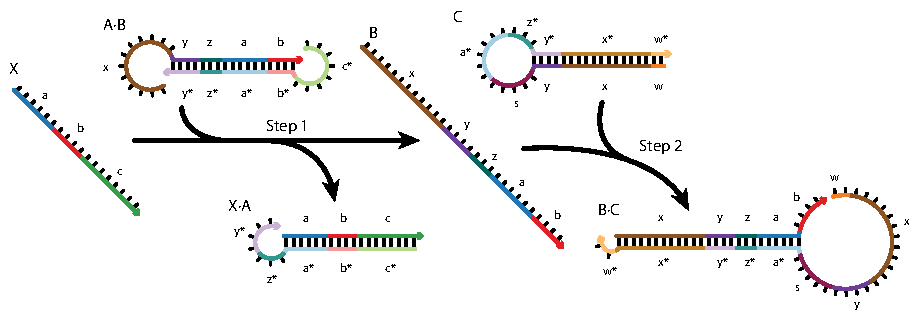
\includegraphics[]{./figs/pathway-dicer}
\bigskip
\begin{footnotesize}
\begin{tabular}{ccp{2.2in}p{2.3in}}
\toprule
Step & Reaction & Function  & Mechanism \\ \midrule
1 & X + A\plex B \unidir  X\plex A + B& detect target X (sequence `a-b-c') & toehold/toehold nucleation, 3-way branch migration, spontaneous dissociation\\
2& B + C \unidir B\plex C  & form Dicer substrate targeting independent target Y (sequence `w-x-y-z') & toehold/loop nucleation, 3-way branch migration\\ 
\bottomrule
\end{tabular}
\end{footnotesize}
\bigskip
\caption{Reaction pathway for conditional Dicer substrate formation via shape and sequence transduction with small conditional RNAs (scRNAs; Hochrein et al., {\it J Am Chem Soc}, 2013). 
scRNA A\plex B detects target X (comprising sequence `a-b-c'), generating intermediate B that assembles with scRNA C to generate Dicer substrate B\plex C (targeting independent sequence `w-x-y-z' for silencing). Top:~Reaction pathway schematic.  Bottom:~Elementary step details. 
\label{fig:dicer-pathway}
    }
\end{figure}



\begin{figure}
\centering
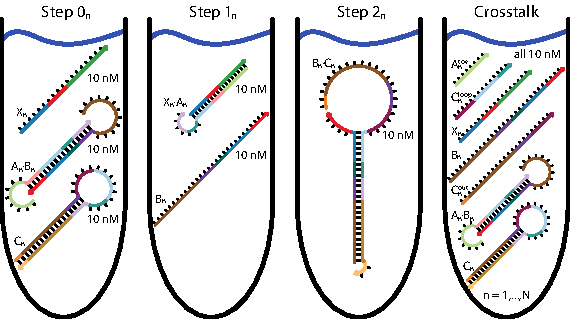
\includegraphics[]{./figs/tubes-dicer}
\bigskip\bigskip
\begin{footnotesize}
\begin{tabular}{lll}
\toprule
Tube & On-targets ($\Psi^{\rm on}_h$)&  Off-targets ($\Psi^{\rm off}_h$) \\ \midrule
Step 0\sub{n} &  \{X, A\plex B, C\}\sub{n}	& \{A, B\plex C\}\sub{n} $\cup~\Psi^{L\le L_{\rm max}}_{0_n}~ -$ \{X\plex A\} \\[3pt]
Step 1\sub{n} &  \{X\plex A, B\}$_n$	& \{X, A\plex B\}\sub{n} $\cup~\Psi^{L\le L_{\rm max}}_{1_n}$ \\[3pt]
Step 2\sub{n} &  \{B\plex C\}$_n$	& \{B, C\}\sub{n} $\cup~\Psi^{L\le L_{\rm max}}_{2_n}$\\[3pt]
Crosstalk & $\cup_{n=1,\dots,N}\{\lambda_n^{\rm reactive}$\} & $\Psi^{L\le L_{\rm max}}_{\rm global} - \cup_{n=1,\dots,N}\{\lambda_n^{\rm cognate}\}$\\
 \bottomrule
\end{tabular}
\end{footnotesize}
\bigskip
\caption{
Target test tubes for conditional Dicer substrate formation via shape and sequence transduction with scRNAs.
Top:~Target test tube schematics. Bottom:~Target test tube details. 
Each target test tube contains the depicted on-target complexes (each with the depicted target structure and a target concentration of 10 nM) 
and the off-target complexes listed in the table (each with vanishing target concentration). To simultaneously design $N$ orthogonal systems, the total number of target test tubes is $|\Omega| = 3N + 1$. $L_{\rm max} = 2$ for all tubes. Design conditions: RNA in 1 M Na$^+$ at 37 $^\circ$C.
        \label{fig:dicer-tubes}
    }
\end{figure}
\bigskip



\end{document}